\subsubsubsection{Registrovanje snabdevača}

\begin{itemize}
	\item Kratak opis:
		\begin{itemize}
			\item Administrator pravi nalog novom snabdevaču.
		\end{itemize}
	\item Učesnici:
		\begin{itemize}
			\item Snabdevač
			\item Administrator
		\end{itemize}				
	\item Preduslovi:
		\begin{itemize}
		    \item Snabdevač je popunio prijavu.
		    \item Administrator je dobio od inspekcije izveštaj i propratnu dokumentaciju snabdevača. %idk if this is a thing
		    \item Sistem je u funkciji.
		\end{itemize}
	\item Postuslovi:
		\begin{itemize}
			\item U bazu je ubačen snabdevač i omogućeno mu je da pristupa novonapravljenom nalogu.
		\end{itemize}		
	\item Osnovni tok:
		\begin{enumerate}
		    \item Administrator proverava da li snabdevač ispunjava neophodne uslove analizirajući izveštaj inspekcije i propratnu dokumentaciju snabdevača.
		    \item Administrator pristupa sistemu i bira opciju za generisanje ugovora. 
		    \item Sistem generiše ugovor.
		    \item Administrator šalje mejl novom snabdevaču koji sadrži ugovor i zahtev da ga potpiše.
		    \item Snabdevač potpisuje i šalje ga nazad.
		    \item Administrator bira opciju za pravljenje novog naloga i pravi nalog novom snabdevaču na osnovu prijave snadbdevača.
		    \item Administrator arhivira dokumentaciju snabdevača i izveštaj inspekcije.
		    \item Sistem trajno čuva prijavu snabdevača.
		    \item Sistem šalje mejl novom snabdevaču o uspešnoj registraciji i kaže mu da aktivira svoj nalog tako što će uneti ponudu.
		   \item Snabdevač se prijavljuje po prvi put i unosi svoju trenutnu ponudu.
		\end{enumerate}
	\item Alternativni tok:
		\begin{itemize}
			 \item[1.a] Snabdevač ne ispunjava zahtevane uslove. Njegova prijava je odbijena i trajno se čuva u bazi. Ne može podneti novu prijavu u narednih 6 meseci. Slučaj korišćenja se završava.
		  %  \item[4.a] Snabdevač nije pripremio potrebnu dokumentaciju prilikom inspekcije. U tom slučaju određuje se novi termin za inspekciju. Slučaj korišćenja se nastavlja od koraka 4.
	
		\end{itemize}
	\item Dodatne informacije:
		\begin{itemize}
			\item Neophodna dokumenta snabdevača koje administrator dobija od inspekcije pored izveštaja podrazumevaju izvod iz Registra poljoprivrednih gazdinstava ili izvod iz Agencije za privredne registre.
		\end{itemize}						
\end{itemize}

\begin{figure}[H]
\begin{center}
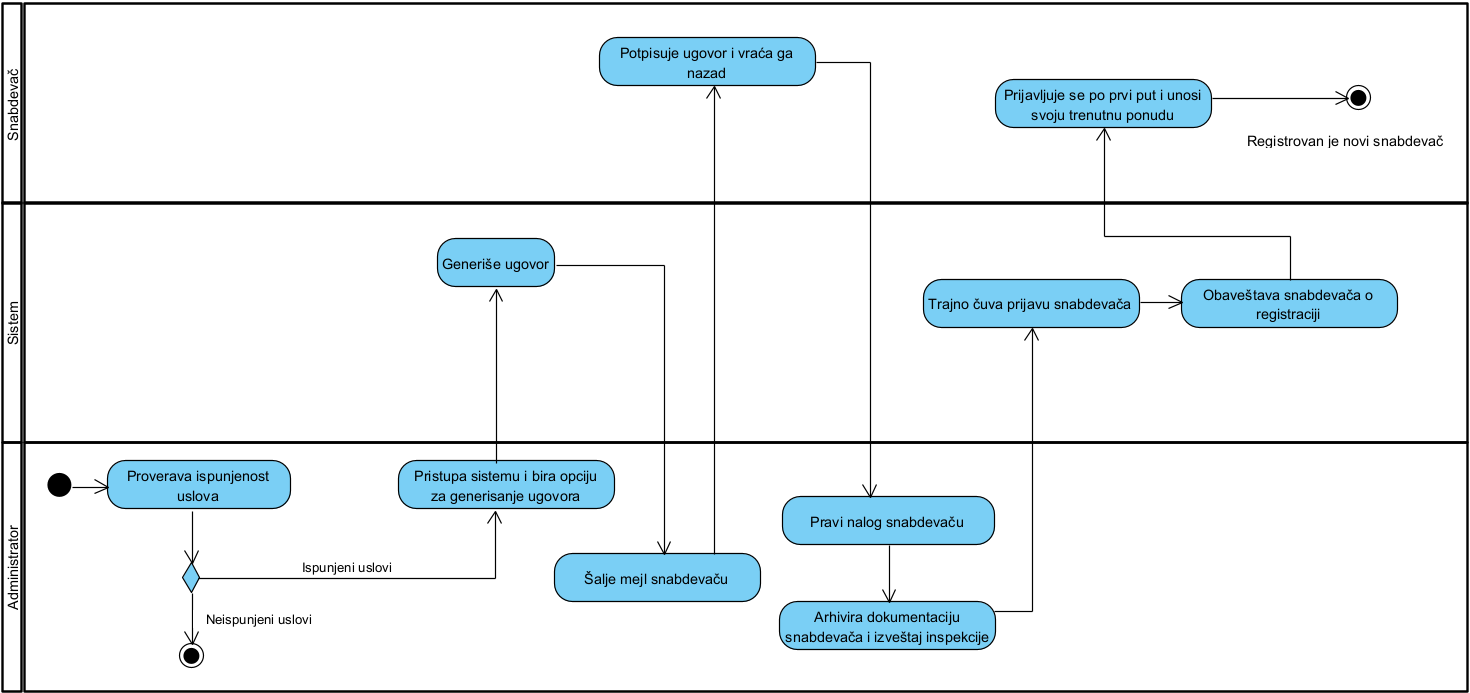
\includegraphics[width=\textwidth]{Pictures/activity_supplier_registration.png}
\end{center}
    \caption{Dijagram aktivnosti registrovanja snabdevača}
\label{fig:ActivitySupplierRegistration}
\end{figure}